\subsection{Methodology}

In this project we have decided to use an adaption of the SCRUM-methodology, an
agile methodology. We chose this method because of the highly volatile nature
of requirements. The project description and domain is very loosely defined,
and we expect the requirements to change significantly during the development
of the application. In addition, the customer and the advisor from IDI
recommended we used an agile methodology.

However, as previously stated, we will use an adaption of the SCRUM
methodology. We will perform daily standups, use sprint planning, have a
product owner and a scrum master. However, we will not strictly employ
standards such as SCRUM board. We will also be agile in our use of the sprint
plan, taking into consideration the ever changing requirements.

% Maybe some notes about why the course makes it problematic to follow strict
% SCRUM due to their waterfall-oriented documentation requirements

\subsection{Project phases}

Our project will loosely follow the plan in Figure~\ref{gantt:project}.

\begin{figure}[h]
\centering
  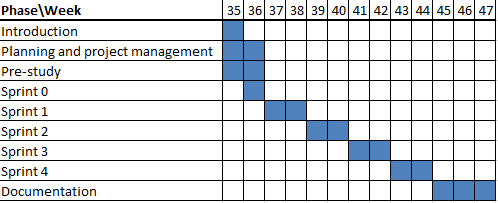
\includegraphics[width=1.0\textwidth]{project_management/project_effort_estimation}
  \caption[Gantt chart of project phases]{Gantt chart showing project phases, and when they are planned done.}
  \label{gantt:project}
\end{figure}

\subsubsection{Planning and research}

This first phase of the project consists of an introduction to the course,
planning of the project, introduction to the problem domain, getting to know
the group, requirement gathering and such. In this phase the most important
decisions about system architecture, choice of COTS and framework, project
% What is COTS?
methodology and role distribution, will be taken. Figure~\ref{gantt:pre_imp}
shows how the work will be distributed in this time period.

\begin{figure}[h]
\centering
  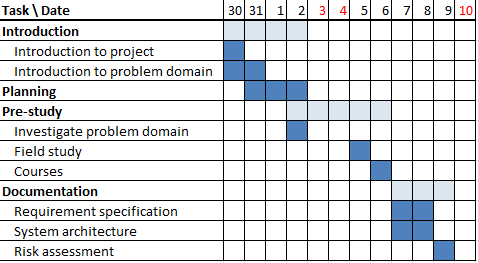
\includegraphics[width=1.0\textwidth]{project_management/pre_implementation_gantt}
  \caption[Gantt chart of planning and research phase]{Gantt diagram picturing how work should be distributed in the time available during the planning and research phase.}
  \label{gantt:pre_imp}
\end{figure}

\subsubsection{Sprints}

Each sprint will consist of four phases. Effort estimation is
detailed in Table \ref{Sprint effort estimation}.

\begin{table}[htbp]
\begin{center}
  \begin{tabular}{|r|r|r|}
    \hline
    \bf{Task} & \bf{Hours per person} & \bf{Hours total} \\
    \hline
    Planning & 8 & 56 \\
    Implementation & 8 & 56 \\
    Testing & 8 & 56 \\
    Documentation & 16 & 112 \\
    Administrative & 8 & 56 \\
    \hline \hline
    \bf{Sum} & 50 & 350 \\
    \hline
  \end{tabular}
  \caption{Task effort estimation for each sprint}
  \label{Sprint effort estimation}
\end{center}
\end{table}

\textbf{Planning} The planning phase of each sprint represents the time
required for work distribution, planning of how each task should be handled,
and how testing should be done for this section.

\textbf{Implementation} The implementation phase represents time spent on coding.
This will also include code refactoring and other maintenance tasks
related to the code.

\textbf{Testing} The testing phase represents time spent testing the system.
This includes integration testing, unit testing, functional testing etc.
The testing and implementation phases will work concurrently due to the
test-driven development methodology.

\textbf{Documentation} The documentation phase represents time spent
documenting work effort (implementation, research, etc.) and administrative
tasks like meetings.
